\chapter{Inovação Social no Território: Economia Solidária, Bioeconomia e Indicações Geográficas}
\label{cap:unid1_cap06}

\noindent\tagAV{AV1 (30\%)}\ \tagTerritorio

\vspace{6pt}

\begin{capObjetivos}
Ao concluir este capítulo, você deverá ser capaz de:
\begin{itemize}[leftmargin=1.4em, itemsep=3pt]
  \item Explicar por que nem toda tecnologia funciona em todo território, diferenciando \textbf{Tecnologia Convencional (TC)} e \textbf{Tecnologia Social (TS)} via \textbf{Adequação Sociotécnica} (Dagnino, 2014).
  \item Compreender os princípios da \textbf{Economia Solidária} e da \textbf{autogestão}, incluindo a lógica de distribuição de sobras produtivas.
  \item Analisar a \textbf{bioeconomia territorial} e as cadeias da sociobiodiversidade como alternativas ao extrativismo primário exportador.
  \item Distinguir as modalidades de \textbf{Indicações Geográficas (IGs)} no Brasil (Lei n.\textsuperscript{o} 9.279/1996, INPI): \textbf{Indicação de Procedência (IP)} e \textbf{Denominação de Origem (DO)}, aplicando exemplos baianos.
  \item Calcular o \textbf{prêmio de preço territorial ($\pi_{IG}$)}, o \textbf{ganho líquido unitário} e a \textbf{Retenção de Valor Local ($RVL$)}, integrando toda a Unidade I para o Seminário e Fichamento Crítico da \textbf{AV1 (30\%)}.
\end{itemize}
\end{capObjetivos}

\begin{capRevisao}
Nos Capítulos~1 a~5, percorremos a trajetória teórica da destruição criadora e da espacialidade (Cap.~1), das aglomerações produtivas e barreiras de entrada (Cap.~2), dos ecossistemas e proximidades (Cap.~3), da governança em Hélice Quíntupla e políticas públicas (Cap.~4) e dos negócios híbridos de impacto (Cap.~5). Neste Capítulo~6, fechamos a Unidade~I examinando como territórios constroem inovação \textbf{a partir de baixo}, combinando tecnologia social, autogestão, sociobiodiversidade e proteção jurídica da origem via Indicações Geográficas.
\end{capRevisao}

\etapa{3}{Fundamentação Teórica, Propriedade Intelectual Territorial e Modelagem}

\begin{boxSimbolo}[Vocabulário Conceitual e Símbolos do Capítulo]
\renewcommand{\arraystretch}{1.18}
\begin{tabular}{@{}p{2.4cm} p{12.0cm}@{}}
  TC / TS & Tecnologia Convencional vs. Tecnologia Social. \\
  AST & Adequação Sociotécnica (adaptação participativa de artefatos e processos ao contexto local). \\
  IG / IP / DO & Indicação Geográfica / Indicação de Procedência / Denominação de Origem (Lei 9.279/1996). \\
  $P_{IG},\ P_{comm}$ & Preço obtido com Indicação Geográfica vs. preço de referência como \textit{commodity}. \\
  $\pi_{IG}$ & Prêmio percentual de preço territorial conferido pela IG. \\
  $C_{cert},\ Q$ & Custo anual fixo de certificação/rastreabilidade e volume comercializado (kg, L ou sacas). \\
  $G_{unit}$ & Ganho líquido unitário após descontar o custo de certificação por unidade. \\
  $RVL$ & Taxa de Retenção de Valor Local ($V_{remunerado\_local} / V_{bruto\_final}$). \\
\end{tabular}
\end{boxSimbolo}

\subsection{Por que Nem Toda Tecnologia Funciona em Todo Território? Tecnologia Convencional vs. Tecnologia Social}

A visão tradicional assume que a ciência e a tecnologia são neutras e universais, pressupondo que bastaria transferir uma máquina eficiente de um país central para uma cooperativa rural para gerar desenvolvimento. Renato Dagnino (2014) desmonta essa tese ao mostrar que a \textbf{Tecnologia Convencional (TC)} é moldada pelos valores da empresa capitalista de grande escala, pois busca poupar mão de obra, exige grandes volumes de capital, depende de insumos sintéticos externos, segmenta o trabalho e concentra decisões na gerência. Quando inserida sem mediação em territórios de agricultura familiar ou economia popular, a TC frequentemente quebra financeiramente o empreendimento ou gera dependência técnica contínua.

Em contraposição, a \textbf{Tecnologia Social (TS)} compreende produtos, técnicas ou metodologias reaplicáveis, desenvolvidas na interação com a comunidade e que representam efetivas soluções de transformação social. Seu processo central consiste na \textbf{Adequação Sociotécnica (AST)}, entendida como o redesenho participativo de tecnologias existentes (ou a criação de novas) para compatibilizá-las com a escala produtiva, os saberes locais, a disponibilidade energética e a propriedade coletiva do território.

\subsection{Economia Solidária, Autogestão e Bioeconomia Territorial}

A \textbf{Economia Solidária}, sistematizada no Brasil por Paul Singer, organiza a produção com base na \textbf{autogestão}, arranjo em que os trabalhadores atuam simultaneamente como proprietários coletivos e gestores democráticos de cooperativas, associações e bancos comunitários. Diferentemente do lucro apropriado por acionistas externos, o excedente econômico recebe o nome de \textbf{sobras}, que, após deduções legais (como o Fundo de Reserva e o Fundo de Assistência Técnica, Educacional e Social, FATES), são distribuídas proporcionalmente ao trabalho ou à produção entregue por cada associado.

Quando articulada à \textbf{Bioeconomia Territorial}, a economia solidária supera o modelo de extrativismo primário exportador. Ao transcender a venda de matéria-prima bruta da sociobiodiversidade (como amêndoas, frutos da Caatinga ou óleos vegetais) a preços deprimidos, as redes locais internalizam etapas de beneficiamento, rastreabilidade e agroindustrialização, convertendo patrimônio biocultural em renda retida no território.

\subsection{Indicações Geográficas (IGs) no Brasil e Valorização do \textit{Terroir}}

No Brasil, a Lei da Propriedade Industrial (Lei n.\textsuperscript{o} 9.279/1996), operacionalizada pelo Instituto Nacional da Propriedade Industrial (INPI), protege a reputação e as qualidades vinculadas ao território por meio das \textbf{Indicações Geográficas (IGs)}, entendidas como ativos coletivos pertencentes ao conjunto dos produtores locais em regime de titularidade compartilhada. A legislação brasileira distingue duas modalidades principais de proteção territorial.

\begin{boxConceito}[Indicação de Procedência (IP) vs. Denominação de Origem (DO)]
A \textbf{Indicação de Procedência (IP, art. 177)} protege o nome geográfico de um país, cidade, região ou localidade que tenha se tornado \textbf{conhecido (notoriedade)} como centro de extração, produção ou fabricação de determinado produto ou prestação de serviço, exigindo comprovação histórica de reputação e caderno de especificações técnicas. Por sua vez, a \textbf{Denominação de Origem (DO, art. 178)} exige um nexo causal mais rigoroso, pois protege o nome geográfico cujo produto ou serviço possua qualidades ou características que se devam \textbf{exclusiva ou essencialmente ao meio geográfico}, incluídos fatores naturais (solo, clima, altitude, microrganismos) e fatores humanos (saber-fazer tradicional), conjunto conceituado como \textbf{\textit{terroir}}.
\end{boxConceito}

Na Bahia, o uso estratégico de IGs ilustra como a diferenciação territorial cria barreiras de entrada contra a concorrência baseada apenas em preço baixo, conectando-se diretamente aos mecanismos de eficiência coletiva. Nesse contexto, o \textbf{Cacau do Sul da Bahia (IP)} valoriza o sistema agroflorestal \textit{cabruca} e a qualidade pós-colheita por fermentação controlada para o mercado de chocolates especiais (\textit{bean-to-bar}), enquanto a \textbf{Cachaça da Microrregião de Abaíra (IP)} protege o saber-fazer secular da Chapada Diamantina e eleva o valor agregado da produção artesanal familiar. De modo complementar, o \textbf{Café da Chapada Diamantina e do Oeste da Bahia} exemplifica a segmentação entre cafés especiais de altitude com forte identidade de \textit{terroir} e cafés de alta tecnificação irrigada, ambos buscando diferenciação de origem. A Figura~\ref{fig:tecnologia_social_igs} integra esses três vetores ao esquematizar como a Tecnologia Social, a Economia Solidária, a Bioeconomia e as Indicações Geográficas convergem para ampliar a Retenção de Valor Local ($RVL$).

\begin{figure}[H]
  \centering
  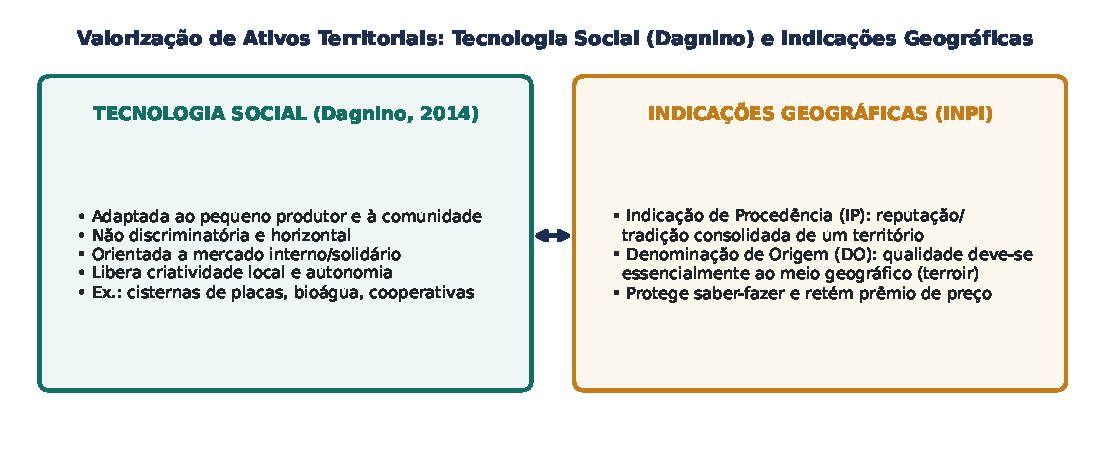
\includegraphics[width=0.94\textwidth]{figures/fig06_tecnologia_social_igs.pdf}
  \caption{Articulação entre Tecnologia Social, Economia Solidária, Bioeconomia e Indicações Geográficas para ampliação da Retenção de Valor Local ($RVL$).}
  \label{fig:tecnologia_social_igs}
\end{figure}

Essa convergência manifesta-se nos territórios baianos, conforme ilustram as subfiguras (a), (b) e (c) da Figura~\ref{fig:igs_tecnologia_bahia}.

\begin{figure}[H]
  \centering
  \begin{minipage}[t]{0.31\textwidth}
    \centering
    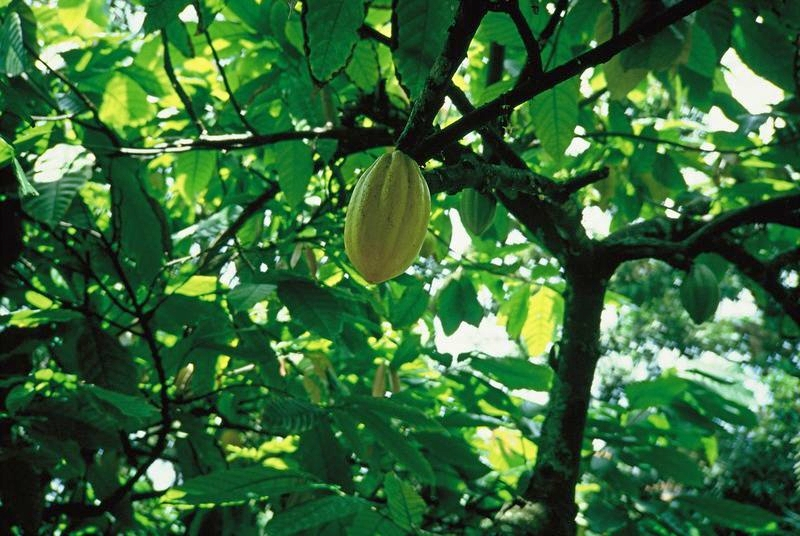
\includegraphics[width=\textwidth,height=3.4cm,keepaspectratio]{figures/foto_cacau_ilheus.jpg}
    \par\small\textbf{(a)} Cacau cultivado no Sul da Bahia (Ilhéus): base para Indicação de Procedência.
  \end{minipage}\hfill
  \begin{minipage}[t]{0.31\textwidth}
    \centering
    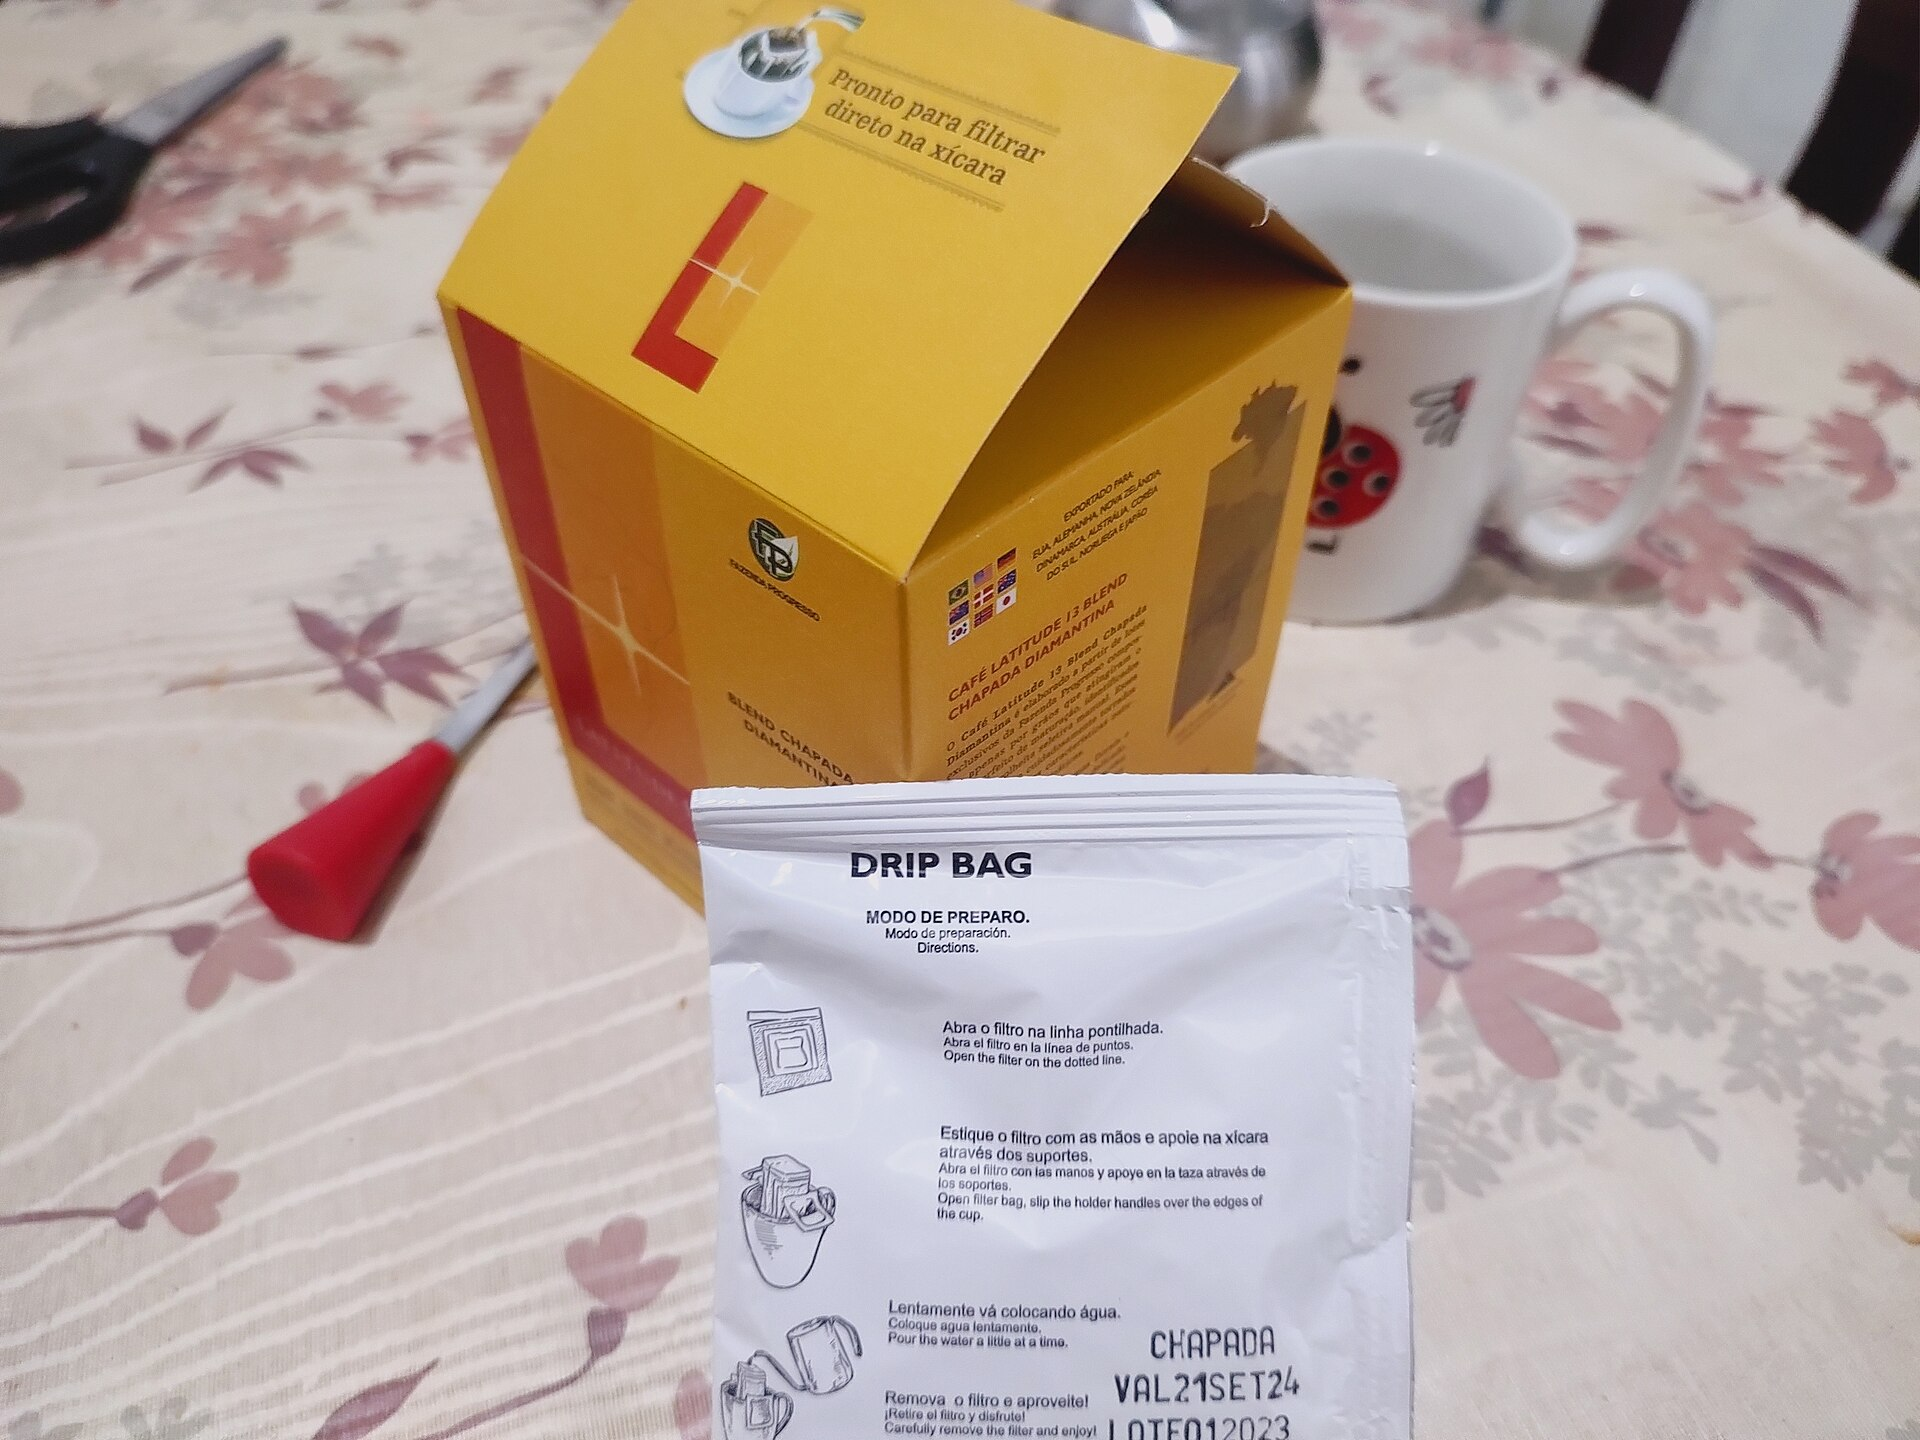
\includegraphics[width=\textwidth,height=3.4cm,keepaspectratio]{figures/foto_cafe_chapada_diamantina.jpg}
    \par\small\textbf{(b)} Café especial de Mucugê na Chapada Diamantina: diferenciação por \textit{terroir}.
  \end{minipage}\hfill
  \begin{minipage}[t]{0.31\textwidth}
    \centering
    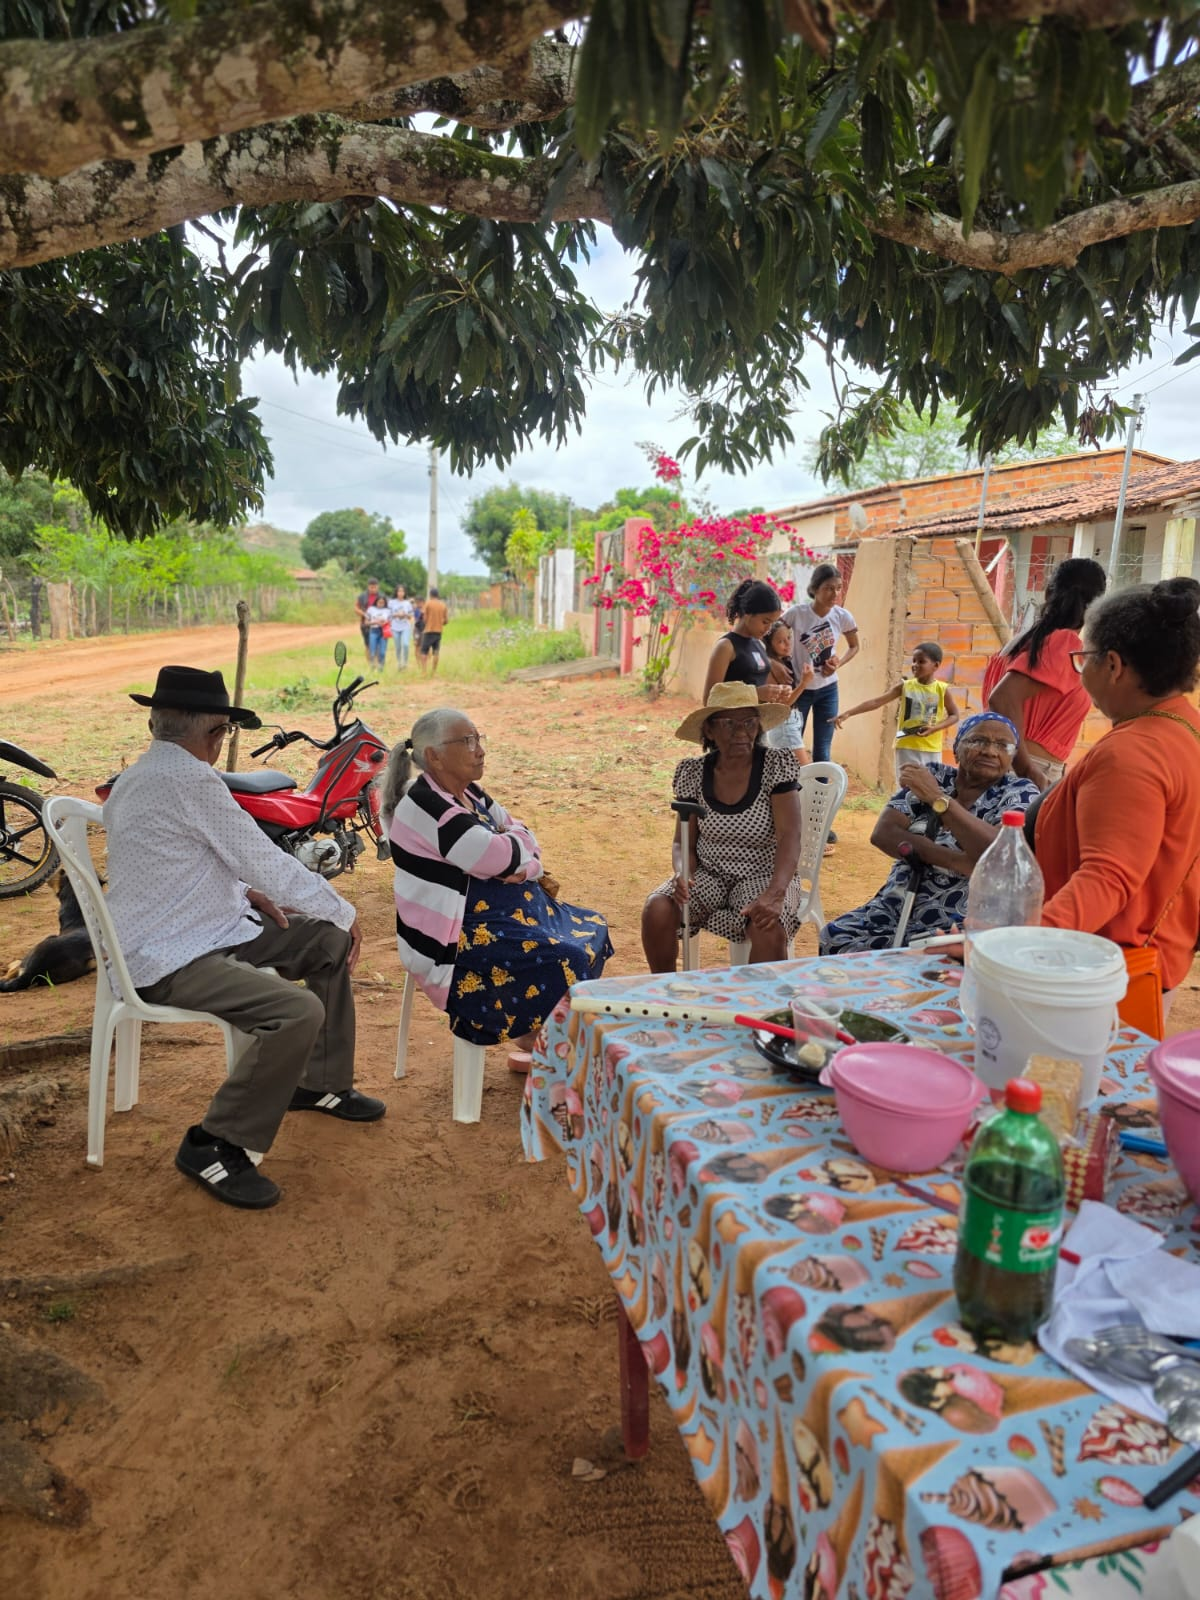
\includegraphics[width=\textwidth,height=3.4cm,keepaspectratio]{figures/foto_quilombo_territorio.jpg}
    \par\small\textbf{(c)} Organização comunitária quilombola em Tranqueira (BA): tecnologia social e território.
  \end{minipage}
  \caption{\textbf{Expressões de diferenciação territorial e tecnologia social na Bahia.} \textit{O que observar:} em (a) e (b), produtos vinculados à origem geográfica substituem a lógica de \textit{commodity} indiferenciada por prêmio de qualidade territorial. Em (c), a organização coletiva em comunidade quilombola exemplifica a retenção de valor apoiada em governança local e saberes tradicionais. Fonte: Wikimedia Commons, CC BY/CC BY-SA (a, b) e Projeto Catuxe/UEFS (c).}
  \label{fig:igs_tecnologia_bahia}
\end{figure}

\begin{boxFormula}[Prêmio de Preço Territorial, Ponto de Equilíbrio e Retenção de Valor Local]
\textbf{1. Prêmio Percentual de Preço Territorial ($\pi_{IG}$):}
\[
\pi_{IG} = \left(\frac{P_{IG} - P_{comm}}{P_{comm}}\right) \times 100\%
\]

\textbf{2. Ganho Líquido Unitário da Certificação ($G_{unit}$) e Volume de Equilíbrio ($Q^*$):}
Considerando o custo anual fixo de governança, rastreabilidade e auditoria da IG ($C_{cert}$) para um volume comercializado $Q$:
\[
G_{unit} = (P_{IG} - P_{comm}) - \frac{C_{cert}}{Q} \qquad \text{e} \qquad Q^* = \frac{C_{cert}}{P_{IG} - P_{comm}}
\]
A IG só gera ganho econômico líquido quando $Q > Q^*$.

\textbf{3. Taxa de Retenção de Valor Local ($RVL$):}
Mede a fração do preço final pago pelo consumidor que efetivamente remunera trabalho, renda e fornecedores dentro do território:
\[
RVL = \left(\frac{V_{remunerado\_local}}{V_{bruto\_final}}\right) \times 100\%
\]
\end{boxFormula}

\subsection{Síntese Integradora para a AV1 (30\%): Seminário e Fichamento Crítico}

A avaliação da Unidade~I (\textbf{AV1, 30\%}) exige que você integre os seis capítulos em um diagnóstico territorial coerente. Um bom fichamento crítico ou seminário deve articular o paradigma tecnológico e o espaço geográfico (Cap.~1) com as barreiras de entrada e a eficiência coletiva (Cap.~2), identificando as lacunas de proximidade e a estrutura do ecossistema local (Cap.~3). A partir dessa base, a análise avança para a governança em hélice e as políticas de CT\&I (Cap.~4), incorpora a arquitetura de impacto e o risco de \textit{mission drift} (Cap.~5) e culmina nas estratégias de adequação sociotécnica, economia solidária e proteção de origem territorial (Cap.~6).

\etapa{4}{Exemplos Resolvidos e Estudos de Caso Comentados}

\begin{boxExemplo}{6.1}{Adequação Sociotécnica no Beneficiamento do Umbu e do Licuri}
\passoEnunciado{Uma cooperativa de mulheres extrativistas no Semiárido recebeu, via doação, uma linha industrial importada de processamento de polpa dimensionada para $10$ toneladas/hora, movida a energia trifásica de alta potência.}
\passoDados{A comunidade produz no máximo $1{,}2$ tonelada/dia na safra sazonal, dispõe de rede elétrica rural monofásica instável e não possui técnicos externos para manutenção de placas eletrônicas proprietárias.}
\passoPedido{Diagnosticar por que a Tecnologia Convencional (TC) falhou no território e propor uma solução de Tecnologia Social (TS) baseada em Adequação Sociotécnica (AST).}
\passoMetodo{Aplicação dos critérios de Adequação Sociotécnica de Renato Dagnino (escala, matriz energética, autonomia de manutenção e controle coletivo).}
\passoContas{
1. Diagnóstico da TC: superdimensionamento ($10\text{ t/h}$ vs. oferta de $1{,}2\text{ t/dia}$ gera ociosidade superior a $95\%$ e custo fixo impagável); incompatibilidade elétrica; caixa-preta tecnológica dependente de peças importadas.\\
2. Redesenho via AST: adoção de despolpadeiras modulares de aço inox em pequena escala ($150\text{ kg/h}$ cada), alimentadas por sistema solar fotovoltaico descentralizado e com mecânica aberta passível de manutenção por serralheiros e eletricistas do próprio município.
}
\passoResposta{A TC geraria endividamento e paralisação; a TS via módulos solares descentralizados ajusta escala, energia e autonomia técnica à realidade da cooperativa.}
\passoVerificacao{O exemplo ilustra que eficiência técnica abstrata (litros ou toneladas por hora) não equivale à eficiência econômica e territorial.}
\end{boxExemplo}

\begin{boxExemplo}{6.2}{Distribuição de Sobras em Cooperativa Solidária Autogestionária}
\passoEnunciado{Uma cooperativa agroextrativista solidária encerrou o exercício anual e precisa deliberar em assembleia sobre a destinação de suas sobras líquidas.}
\passoDados{Receita bruta anual: $\reais{480.000,00}$. Custos operacionais e despesas administrativas totais: $\reais{330.000,00}$. O estatuto prevê destinação de $10\%$ da sobra bruta para o Fundo de Reserva e $5\%$ para o FATES (assistência técnica e educação cooperativista). O total de horas trabalhadas pelo conjunto dos cooperados no ano foi de $42.500\text{ h}$.}
\passoPedido{Calcular a sobra bruta, os valores retidos nos fundos coletivos, a sobra distribuível e o rateio correspondente a uma cooperada que trabalhou $1.800\text{ h}$ no ano.}
\passoMetodo{Apuração contábil cooperativista (Lei n.\textsuperscript{o} 5.764/1971) e rateio proporcional ao trabalho.}
\passoContas{
1. Sobra bruta: $S_{bruta} = 480.000 - 330.000 = \reais{150.000,00}$.\\
2. Retenções estatutárias: Fundo de Reserva ($10\%$) $= \reais{15.000,00}$; FATES ($5\%$) $= \reais{7.500,00}$. Total retido $= \reais{22.500,00}$.\\
3. Sobra distribuível:
\[
S_{dist} = 150.000 - 22.500 = \reais{127.500,00}
\]
4. Valor por hora trabalhada e cota da cooperada ($1.800\text{ h}$):
\[
v_h = \frac{127.500}{42.500} = \reais{3,00}/\text{hora} \implies \text{Cota} = 1.800 \times 3{,}00 = \reais{5.400,00}
\]
}
\passoResposta{A sobra distribuível é de $\reais{127.500,00}$ ($\reais{3,00}/\text{hora}$), cabendo $\reais{5.400,00}$ à cooperada, além de $\reais{22.500,00}$ reinvestidos na resiliência e formação coletiva.}
\passoVerificacao{Diferentemente de sociedades anônimas que remuneram o capital investido, a cooperativa remunera o trabalho efetivo e fortalece reservas indivisíveis do território.}
\end{boxExemplo}

\begin{boxExemplo}{6.3}{Prêmio de Preço Territorial e Ponto de Equilíbrio no Cacau do Sul da Bahia}
\passoEnunciado{Uma associação de produtores agroflorestais avalia aderir ao selo de Indicação de Procedência (IP) do Cacau do Sul da Bahia para comercializar amêndoas fermentadas finas.}
\passoDados{Preço de referência do cacau \textit{commodity}: $P_{comm} = \reais{18,00}/\text{kg}$. Preço alcançado com o selo IP e rastreabilidade: $P_{IG} = \reais{27,00}/\text{kg}$. Custo anual fixo de auditoria, selos e governança da associação para esse grupo: $C_{cert} = \reais{36.000,00}/\text{ano}$. Produção anual comercializada pelo grupo: $Q = 12.000\text{ kg/ano}$.}
\passoPedido{Calcular o prêmio percentual de preço ($\pi_{IG}$), o ganho líquido unitário ($G_{unit}$) e o volume mínimo de equilíbrio ($Q^*$).}
\passoMetodo{Aplicação das equações de prêmio territorial e ponto de equilíbrio de certificação.}
\passoContas{
1. Prêmio percentual de preço:
\[
\pi_{IG} = \left(\frac{27{,}00 - 18{,}00}{18{,}00}\right) \times 100\% = \frac{9{,}00}{18{,}00} \times 100\% = 50{,}0\%
\]
2. Custo de certificação por quilograma e ganho líquido unitário:
\[
\frac{C_{cert}}{Q} = \frac{36.000}{12.000} = \reais{3,00}/\text{kg} \implies G_{unit} = (27{,}00 - 18{,}00) - 3{,}00 = \reais{6,00}/\text{kg}
\]
3. Volume mínimo de equilíbrio ($Q^*$):
\[
Q^* = \frac{36.000}{27{,}00 - 18{,}00} = \frac{36.000}{9{,}00} = 4.000\text{ kg/ano}
\]
}
\passoResposta{O prêmio de preço é de $50{,}0\%$, gerando ganho líquido de $\reais{6,00}/\text{kg}$ ($\reais{72.000,00}/\text{ano}$ adicionais). O grupo opera bem acima do ponto de equilíbrio de $4.000\text{ kg/ano}$.}
\passoVerificacao{O resultado explica por que pequenos produtores individuais não conseguem arcar sozinhos com custos fixos de certificação ($C_{cert}$): a governança coletiva é condição econômica para diluir o custo fixo.}
\end{boxExemplo}

\begin{boxExemplo}{6.4}{Retenção de Valor Local ($RVL$) no Café da Chapada Diamantina}
\passoEnunciado{Compare duas estratégias de inserção comercial para o café especial produzido por uma cooperativa da Chapada Diamantina: venda como grão verde \textit{commodity} para exportadoras externas versus torrefação e embalagem própria com selo de Indicação Geográfica.}
\passoDados{Preço final médio pago pelo consumidor no varejo nacional: $V_{bruto\_final} = \reais{60,00}/\text{kg}$.\\
\textbf{Cenário A (grão verde sem marca territorial):} cooperativa vende o quilo a $\reais{22,00}$ para intermediário externo; insumos químicos externos consumidos na lavoura somam $\reais{10,00}/\text{kg}$.\\
\textbf{Cenário B (café torrado, embalado e certificado com IG local):} cooperativa vende diretamente ou via varejo parceiro retendo $\reais{54,00}/\text{kg}$ no território; insumos e embalagens adquiridos de fora do território somam $\reais{14,00}/\text{kg}$.}
\passoPedido{Calcular o valor líquido retido no território por quilograma e a Taxa de Retenção de Valor Local ($RVL$) em ambos os cenários.}
\passoMetodo{Cálculo de $V_{remunerado\_local} = \text{Receita local} - \text{Insumos externos}$ e razão $RVL = (V_{remunerado\_local}/V_{bruto\_final}) \times 100\%$.}
\passoContas{
\textbf{Cenário A (\textit{commodity}):}
\[
V_{local, A} = 22{,}00 - 10{,}00 = \reais{12,00}/\text{kg} \implies RVL_A = \left(\frac{12{,}00}{60{,}00}\right) \times 100\% = 20{,}0\%
\]
\textbf{Cenário B (agroindustrialização territorial + IG):}
\[
V_{local, B} = 54{,}00 - 14{,}00 = \reais{40,00}/\text{kg} \implies RVL_B = \left(\frac{40{,}00}{60{,}00}\right) \times 100\% \approx 66{,}7\%
\]
}
\passoResposta{A transição para torrefação local com IG eleva a retenção de valor de $\reais{12,00}/\text{kg}$ ($RVL = 20{,}0\%$) para $\reais{40,00}/\text{kg}$ ($RVL = 66{,}7\%$), mais que triplicando a renda retida no território.}
\passoVerificacao{O cálculo materializa a epígrafe da apostila: internalizar etapas industriais e proteger a origem impede o vazamento de valor agregado para fora da região.}
\end{boxExemplo}

\begin{boxExemplo}{6.5}{Roteiro Integrador da AV1: Caso da Cachaça de Abaíra}
\passoEnunciado{Para o Seminário da AV1, um grupo analisa a Indicação de Procedência da Cachaça da Microrregião de Abaíra (BA).}
\passoDados{Produção artesanal em alambiques de cobre por pequenos produtores, organizada via associação local (APAMA), com tradição histórica na Chapada Diamantina e desafios de sucessão geracional e tratamento de vinhoto.}
\passoPedido{Integrar os conceitos da Unidade~I (Caps.~2, 4 e 6) para estruturar um diagnóstico territorial sintético da cadeia.}
\passoMetodo{Síntese cruzada de barreiras de entrada (Cap.~2), Hélice Quíntupla (Cap.~4) e IG/Tecnologia Social (Cap.~6).}
\passoContas{
\begin{enumerate}[leftmargin=1.4em, itemsep=2pt]
  \item \textbf{Barreiras e Eficiência Coletiva (Cap.~2):} a IP cria uma barreira de entrada por diferenciação territorial impossível de ser copiada por destilarias industriais de grande escala; a associação dilui custos de engarrafamento e controle de qualidade.
  \item \textbf{Hélice Quíntupla (Cap.~4):} integração entre produtores, universidades/IFs (padronização fermentativa e aproveitamento do vinhoto para fertirrigação/biogás, Hélice 5), governo (FAPs e extensão rural) e turismo cultural local (Hélice 4).
  \item \textbf{Tecnologia Social e IG (Cap.~6):} preservação do saber-fazer artesanal com adequação sociotécnica sanitária, evitando descaracterização industrial.
\end{enumerate}
}
\passoResposta{O diagnóstico integra diferenciação de mercado, governança participativa e proteção jurídica coletiva do \textit{terroir}, atendendo integralmente à rubrica analítica da AV1.}
\passoVerificacao{A articulação entre capítulos transforma conceitos isolados em estratégia prática de desenvolvimento territorial.}
\end{boxExemplo}

\etapa{5}{Armadilhas Conceituais e Erros Mais Comuns}

\begin{boxErro}[Erro 1: Confundir Indicação de Procedência (IP) com Denominação de Origem (DO)]
Embora ambas sejam Indicações Geográficas registradas no INPI, a \textbf{IP} baseia-se na \textit{notoriedade} da região como centro produtor, enquanto a \textbf{DO} exige comprovação técnico-científica de que as características do produto decorrem essencial ou exclusivamente do meio geográfico (fatores naturais + humanos).
\end{boxErro}

\begin{boxErro}[Erro 2: Tratar a Indicação Geográfica como Marca Privada]
Uma marca comercial pertence a uma empresa específica e pode ser vendida ou licenciada a qualquer fábrica fora da região. A IG é um \textbf{direito coletivo de uso} vinculado ao território delimitado e ao cumprimento do caderno de especificações técnicas; ninguém de fora da área demarcada pode utilizá-la.
\end{boxErro}

\begin{boxErro}[Erro 3: Reduzir Tecnologia Social a ``Tecnologia Pobre ou Improvisada'']
Tecnologia Social não significa gambiarra de baixa qualidade. Exige rigor científico e engenharia aplicada para construir soluções eficientes em pequena escala, com baixo impacto ambiental e controle pelos trabalhadores locais.
\end{boxErro}

\begin{boxErro}[Erro 4: Achar que o Selo de IG Vende Sozinho Sem Governança]
Obter o registro no INPI é apenas o ponto de partida. Sem rastreabilidade efetiva, controle de qualidade contínuo e estratégia comercial coletiva, o selo não gera prêmio de preço ($\pi_{IG} = 0$) e o custo de certificação ($C_{cert}$) torna-se um passivo para os produtores.
\end{boxErro}

\etapa{6}{Exercícios Propostos (Básicos, Intermediários e Objetivos)}

\textbf{Parte A, Exercícios Básicos (Conceituação e Identificação)}

\textbf{1.} Explique a tese de Renato Dagnino sobre a não neutralidade da Tecnologia Convencional (TC) e defina Adequação Sociotécnica (AST).
\espacoResolucao[1.8cm]

\textbf{2.} Qual é a diferença fundamental entre o destino do excedente em uma empresa capitalista tradicional e em uma cooperativa de economia solidária?
\espacoResolucao[1.8cm]

\textbf{3.} Diferencie Indicação de Procedência (IP) de Denominação de Origem (DO) segundo a Lei n.\textsuperscript{o} 9.279/1996.
\espacoResolucao[1.8cm]

\textbf{4.} Cite dois exemplos de produtos baianos com Indicação Geográfica reconhecida (ou em consolidação) e descreva o ativo territorial protegido em cada um.
\espacoResolucao[1.8cm]

\textbf{5.} Por que a bioeconomia territorial se opõe ao modelo de extrativismo primário exportador?
\espacoResolucao[1.8cm]

\textbf{Parte B, Exercícios Intermediários (Modelagem e Análise Quantitativa)}

\textbf{6.} Uma associação de apicultores vende mel comum a $P_{comm} = \reais{20,00}/\text{kg}$. Após conquistar o registro de IG, passa a vender a $P_{IG} = \reais{31,00}/\text{kg}$. O custo fixo anual de auditoria e selos é $C_{cert} = \reais{22.000,00}$ para uma produção anual de $Q = 5.000\text{ kg}$. Calcule $\pi_{IG}$, $G_{unit}$ e $Q^*$.
\espacoResolucao[2.0cm]

\textbf{7.} Um queijo artesanal certificado é vendido no varejo a $V_{bruto\_final} = \reais{80,00}/\text{kg}$. Na venda direta via cooperativa territorial, os produtores retêm $\reais{52,00}/\text{kg}$ líquidos após descontar embalagens e fermentos comprados fora da região. Calcule a Taxa de Retenção de Valor Local ($RVL$).
\espacoResolucao[2.0cm]

\textbf{8.} Uma cooperativa solidária obteve sobra bruta de $\reais{100.000,00}$, destinou $10\%$ ao Fundo de Reserva e $10\%$ ao FATES. Com $20.000$ horas trabalhadas pelos sócios no ano, quanto receberá um cooperado que acumulou $1.500$ horas?
\espacoResolucao[2.0cm]

\textbf{9.} Um projeto de implantação de biodigestores rurais fracassou em um assentamento porque exigia peças importadas e manutenção de empresa sediada a $600\text{ km}$. Proponha três ajustes de Adequação Sociotécnica para viabilizar o projeto.
\espacoResolucao[2.0cm]

\textbf{10.} Estruture um roteiro de 4 etapas para o Fichamento Crítico da AV1 integrando um território de sua escolha aos conceitos de Tecnopolos/Habitats (Cap.~4), Impacto (Cap.~5) e IGs/TS (Cap.~6).
\espacoResolucao[2.0cm]

\textbf{Parte C, Questões Objetivas (Estilo Exame / Concurso, A a E)}

\textbf{11.} Segundo Renato Dagnino (2014), a Tecnologia Convencional frequentemente entra em conflito com empreendimentos de economia solidária porque:
\begin{alternativas}
  \item É gratuita e de código aberto, impedindo a proteção por patentes.
  \item Incorpora valores da grande empresa capitalista, como economia de mão de obra, alta escala e controle hierárquico, incompatíveis com a autogestão.
  \item Exige obrigatoriamente que todos os trabalhadores tenham título de doutorado.
  \item Não pode ser aplicada em ambientes urbanos industriais.
  \item Elimina a necessidade de energia elétrica ou insumos externos.
\end{alternativas}

\textbf{12.} De acordo com a Lei n.\textsuperscript{o} 9.279/1996 (Lei da Propriedade Industrial), a modalidade de Indicação Geográfica que exige comprovação de que as qualidades do produto decorrem exclusiva ou essencialmente do meio geográfico (fatores naturais e humanos) é denominada:
\begin{alternativas}
  \item Patente de Modelo de Utilidade.
  \item Marca de Alto Renome.
  \item Indicação de Procedência (IP).
  \item Denominação de Origem (DO).
  \item Desenho Industrial Coletivo.
\end{alternativas}

\textbf{13.} Uma cooperativa de derivados de mandioca comercializa farinha especial com IG a $\reais{15,00}/\text{kg}$, frente ao preço de $\reais{10,00}/\text{kg}$ da farinha comum. Sabendo que o custo fixo anual de certificação é de $\reais{25.000,00}$, o volume mínimo de equilíbrio ($Q^*$) para que a certificação comece a gerar ganho líquido positivo é de:
\begin{alternativas}
  \item $1.667\text{ kg/ano}$
  \item $2.500\text{ kg/ano}$
  \item $5.000\text{ kg/ano}$
  \item $7.500\text{ kg/ano}$
  \item $10.000\text{ kg/ano}$
\end{alternativas}

\textbf{14.} Sobre os princípios da Economia Solidária e da autogestão, assinale a alternativa \textbf{correta}:
\begin{alternativas}
  \item O poder de voto nas assembleias é proporcional ao capital integralizado por cada sócio.
  \item As sobras distribuíveis são partilhadas conforme critérios definidos coletivamente (como trabalho ou produção entregue), após constituição dos fundos legais.
  \item A propriedade dos equipamentos pertence a um investidor-anjo externo sem vínculo com o trabalho local.
  \item É vedada a formação de redes de cooperação entre empreendimentos solidários.
  \item Os empreendimentos solidários não podem atuar em cadeias da bioeconomia.
\end{alternativas}

\textbf{15.} Em cadeias produtivas da sociobiodiversidade, a elevação da Taxa de Retenção de Valor Local ($RVL$) ocorre principalmente quando o território:
\begin{alternativas}
  \item Exporta matéria-prima bruta sem beneficiamento e importa produtos acabados.
  \item Substitui espécies nativas por monoculturas dependentes de pacotes químicos externos.
  \item Internaliza etapas de beneficiamento, rastreabilidade e diferenciação por origem (como IGs), reduzindo a dependência de intermediários externos.
  \item Elimina cooperativas para concentrar a terra em um único comprador monopsônico.
  \item Adota pacotes tecnológicos convencionais sem adequação sociotécnica.
\end{alternativas}

\etapa{7}{Questões Autorais Estilo Pós-Graduação e Concursos}

\textbf{16. (Estilo Concurso para Analista de Propriedade Industrial, INPI)} Uma associação de produtores de mel de uma região semiárida deseja registrar uma Indicação Geográfica. A região já possui notoriedade histórica pela produção apícola há 40 anos, mas ainda não dispõe de estudos laboratoriais completos que comprovem a correlação exclusiva entre a flora nativa local e parâmetros físico-químicos específicos do mel. Oriente a associação sobre qual modalidade (IP ou DO) deve ser pleiteada inicialmente e quais evidências técnicas e documentais são exigidas.
\espacoResolucao[2.2cm]

\textbf{17. (Estilo Pós-Graduação em Desenvolvimento Territorial)} Analise o paradoxo da ``mercantilização sem retenção'': em diversas regiões, produtos tradicionais conquistam selos de qualidade e prêmios internacionais, mas a maior parte do valor adicionado continua apropriada por torrefadoras, distribuidoras ou marcas sediadas em metrópoles externas. Proponha estratégias combinadas de Tecnologia Social, Economia Solidária e governança de IG para reverter esse vazamento de valor.
\espacoResolucao[2.2cm]

\textbf{18. (Estilo Mestrado Profissional, PLANTERR/UEFS)} Escolha um arranjo produtivo da sociobiodiversidade baiana (ex.: licuri, umbu, piaçava, cacau cabruca ou cachaça artesanal) e redija um plano sintético articulando: (a) um processo de Adequação Sociotécnica; (b) um modelo de governança autogestionária ou híbrida sem \textit{mission drift}; e (c) estimativa conceitual de como a IG eleva o prêmio de preço ($\pi_{IG}$) e a $RVL$.
\espacoResolucao[2.2cm]

\begin{boxDica}[Checklist Final para a Entrega da AV1 (30\%)]
Antes de apresentar seu Seminário ou entregar o Fichamento Crítico da \textbf{AV1}, verifique se sua análise responde a três perguntas-chave da Unidade~I:
\begin{enumerate}[leftmargin=1.4em, itemsep=2pt]
  \item \textbf{Tecnologia e Território:} a solução proposta é compatível com a escala, a cultura e os recursos locais (AST)?
  \item \textbf{Governança:} as cinco hélices estão articuladas sem captura por interesses privados (socialização do risco)?
  \item \textbf{Retenção de Valor:} o modelo amplia a $RVL$ e protege o patrimônio coletivo territorial?
\end{enumerate}
\end{boxDica}

\clearpage
\etapa{8}{Gabarito Comentado dos 18 Exercícios}

\begin{boxGabarito}[Respostas Comentadas: Capítulo 6]
\textbf{1.} Para Dagnino, a TC embute relações sociais capitalistas (alta escala, substituição de trabalho, dependência de insumos externos), não sendo neutra. A AST consiste no processo participativo de adaptar ou redesenhar tecnologias para que se tornem compatíveis com o controle coletivo e a realidade local.

\textbf{2.} Na empresa capitalista, o lucro remunera o capital investido pelos acionistas; na cooperativa solidária, as sobras (após fundos coletivos) retornam proporcionalmente ao trabalho ou à produção entregue pelos cooperados.

\textbf{3.} A Indicação de Procedência (IP) protege a notoriedade/reputação geográfica do local como centro produtor; a Denominação de Origem (DO) exige nexo causal comprovado de que as qualidades do produto devem-se essencial ou exclusivamente ao meio geográfico (fatores naturais e humanos).

\textbf{4.} Cacau do Sul da Bahia (IP, protege a tradição do sistema cabruca e a qualidade das amêndoas) e Cachaça de Abaíra (IP, protege o saber-fazer artesanal da microrregião na Chapada Diamantina).

\textbf{5.} Porque busca internalizar etapas de processamento, conhecimento científico, rastreabilidade e agregação de valor no território de origem, conservando a sociobiodiversidade em pé em vez de exportar matéria-prima bruta a baixo preço.

\textbf{6.} $\pi_{IG} = [(31 - 20)/20] \times 100\% = 55{,}0\%$. Custo unitário de certificação $= 22.000 / 5.000 = \reais{4,40}/\text{kg}$. $G_{unit} = (31 - 20) - 4{,}40 = \reais{6,60}/\text{kg}$. $Q^* = 22.000 / (31 - 20) = 2.000\text{ kg/ano}$.

\textbf{7.} $RVL = (52{,}00 / 80{,}00) \times 100\% = 65{,}0\%$.

\textbf{8.} Retenção total $= 20\%$ ($\reais{20.000,00}$). Sobra distribuível $= \reais{80.000,00}$. Valor por hora $= 80.000 / 20.000 = \reais{4,00}/\text{h}$. Cota do cooperado $= 1.500 \times 4{,}00 = \reais{6.000,00}$.

\textbf{9.} (i) Substituir peças proprietárias por componentes padronizados disponíveis no comércio regional; (ii) capacitar jovens e moradores locais como técnicos de manutenção; (iii) adaptar a capacidade dos biodigestores ao volume real de biomassa de cada unidade familiar.

\textbf{10.} Roteiro sugerido: (1) caracterização produtiva e barreiras do território; (2) mapeamento da Hélice Quíntupla e instrumentos de CT\&I aplicáveis; (3) avaliação de impacto via Teoria da Mudança e risco de \textit{mission drift}; (4) estratégia de AST, autogestão e proteção via IG para maximizar a $RVL$.

\textbf{11. (B)} Dagnino demonstra que a TC não é neutra, pois incorpora objetivos de acumulação e controle hierárquico incompatíveis com a autogestão solidária.

\textbf{12. (D)} A Denominação de Origem (art. 178 da Lei n.\textsuperscript{o} 9.279/1996) exige nexo causal entre as características do produto e o meio geográfico (fatores naturais e humanos).

\textbf{13. (C)} $Q^* = 25.000 / (15 - 10) = 25.000 / 5 = 5.000\text{ kg/ano}$.

\textbf{14. (B)} Na autogestão cooperativista, cada sócio tem um voto (independentemente do capital) e as sobras distribuíveis remuneram o trabalho ou a produção entregue.

\textbf{15. (C)} A retenção de valor local aumenta quando o território internaliza processamento, governança e diferenciação de origem.

\textbf{16.} Deve pleitear inicialmente a \textbf{Indicação de Procedência (IP)}, pois já dispõe de notoriedade histórica de 40 anos como centro produtor. Exigirá: delimitação da área geográfica, regulamento de uso/caderno de especificações técnicas, comprovação documental da reputação (reportagens, registros históricos, feiras) e estrutura de controle pela associação representativa. Futuramente, com estudos polínicos e físico-químicos que comprovem o nexo com o \textit{terroir}, poderá evoluir para DO.

\textbf{17.} Para evitar que o selo apenas valorize o produto nas mãos de terceiros externos, deve-se: (i) exigir no caderno de especificações que etapas críticas de beneficiamento/embalagem ocorram dentro da área demarcada; (ii) constituir agroindústrias cooperativas autogestionárias com tecnologias sociais modulares; (iii) estruturar comercialização direta em redes solidárias e compras públicas territoriais.

\textbf{18.} Resposta aberta integrando o arranjo escolhido: deve detalhar o redesenho sociotécnico de equipamentos (AST), a proteção contra captura por atravessadores (governança cooperativa) e o mecanismo pelo qual o selo de origem converte commodity regional em produto diferenciado com maior $RVL$.
\end{boxGabarito}

\begin{boxResumo}
\begin{itemize}[leftmargin=1.4em, itemsep=3pt]
  \item A \textbf{Tecnologia Social} e a \textbf{Adequação Sociotécnica} (Dagnino) adaptam soluções produtivas à escala, cultura e autonomia dos trabalhadores do território.
  \item A \textbf{Economia Solidária} baseia-se na autogestão e na partilha de sobras proporcionais ao trabalho/produção, fortalecendo reservas coletivas.
  \item As \textbf{Indicações Geográficas} (IP por notoriedade; DO por nexo causal com o \textit{terroir}) são ativos coletivos que geram prêmio de preço ($\pi_{IG}$) e ampliam a \textbf{Retenção de Valor Local ($RVL$)}, desde que o volume supere o ponto de equilíbrio $Q^*$.
\end{itemize}
\end{boxResumo}

\begin{boxTeste}
Julgue os itens a seguir como Verdadeiros (\V) ou Falsos (\F):
\begin{enumerate}[leftmargin=1.6em, itemsep=3pt]
  \item (\quad) A Adequação Sociotécnica defende que toda tecnologia industrial de grande escala deve ser implantada sem alterações em cooperativas rurais.
  \item (\quad) Na Denominação de Origem (DO), exige-se comprovação de que as qualidades do produto decorrem exclusiva ou essencialmente do meio geográfico, incluindo fatores naturais e humanos.
  \item (\quad) Quando o volume comercializado $Q$ é inferior ao ponto de equilíbrio $Q^* = C_{cert}/(P_{IG} - P_{comm})$, o custo fixo de certificação supera o ganho adicional de preço da IG.
  \item (\quad) A internalização de etapas de beneficiamento e embalagem no território reduz a Taxa de Retenção de Valor Local ($RVL$).
\end{enumerate}
\textbf{Gabarito do Checkpoint:} 1. \F \quad 2. \V \quad 3. \V \quad 4. \F \text{ (eleva a } RVL\text{)}
\end{boxTeste}
